\ifdefined\pdfinfoomitdate\pdfinfoomitdate=1\fi
\ifdefined\pdftrailerid\pdftrailerid{}\fi
\documentclass[11pt]{article}
\usepackage[margin=1in]{geometry}
\usepackage[T1]{fontenc}
\usepackage{lmodern}
\usepackage{microtype}
\usepackage{amsmath}
\usepackage{booktabs}
\usepackage{graphicx}
\usepackage{flafter}
\usepackage{array}
\usepackage[numbers,sort&compress]{natbib}
\usepackage[hidelinks]{hyperref}
\setlength{\emergencystretch}{2em}
\setlength{\tabcolsep}{4pt}
\renewcommand{\topfraction}{0.9}
\renewcommand{\bottomfraction}{0.8}
\renewcommand{\textfraction}{0.1}
\renewcommand{\floatpagefraction}{0.7}

\title{Do More Expressive Probes Improve EEG Age Prediction?\\
A Cross-Cohort Study with Frozen REVE}
\author{Dmytro Kozynko\\
\small Independent Researcher\\
\small\href{mailto:dmytro.kozynko@gmail.com}{\texttt{dmytro.kozynko@gmail.com}}}
\date{}
\hypersetup{
  pdftitle={Do More Expressive Probes Improve EEG Age Prediction? A Cross-Cohort Study with Frozen REVE},
  pdfauthor={Dmytro Kozynko},
  pdfsubject={Frozen EEG representation probing},
  pdfkeywords={EEG, foundation models, representation probing, age prediction}
}
% Hand-authored notation and reusable non-empirical text.
\newcommand{\REVE}{REVE}
\newcommand{\HBN}{HBN}
\newcommand{\MIPDB}{MIPDB}
\newcommand{\DeltaPearson}{\ensuremath{\Delta r}}
\newcommand{\MeanLinear}{\texttt{mean\_linear}}
\newcommand{\LayerLinear}{\texttt{mean\_layer\_linear}}
\newcommand{\RichResidual}{\texttt{mean\_rich\_stats\_residual}}
\newcommand{\MultiQuery}{\texttt{multi\_query\_rich\_stats}}

% Generated deterministically; do not edit.
\newcommand{\PrimarySubjects}{75}
\newcommand{\PilotSubjects}{10}
\newcommand{\ExtrapolationSubjects}{20}
\newcommand{\ProbeSeeds}{10}
\newcommand{\ProbeRuns}{40}
\newcommand{\ExternalPredictions}{3000}
\newcommand{\SourceAnalysisHash}{7747a16e\allowbreak{}11629164\allowbreak{}b524b211\allowbreak{}3ab2230d\allowbreak{}26001202\allowbreak{}2fc46f68\allowbreak{}540c7f75\allowbreak{}78c2a3b6}
\newcommand{\PredictionInventoryHash}{3ec0042d\allowbreak{}613fc2d3\allowbreak{}6937d734\allowbreak{}9081beb0\allowbreak{}739c4fb3\allowbreak{}da349e12\allowbreak{}29e17f22\allowbreak{}6e187830}
\newcommand{\BaselinePearson}{0.644}
\newcommand{\BaselineMAE}{3.241}
\newcommand{\BaselineRMSE}{3.961}
\newcommand{\BaselineRSquared}{-0.674}
\newcommand{\BaselineCalibrationIntercept}{-3.172}
\newcommand{\BaselineCalibrationSlope}{1.706}
\newcommand{\LayerLinearPearson}{0.653}
\newcommand{\LayerLinearMAE}{3.297}
\newcommand{\LayerLinearRMSE}{4.008}
\newcommand{\LayerLinearRSquared}{-0.714}
\newcommand{\LayerLinearCalibrationIntercept}{-3.453}
\newcommand{\LayerLinearCalibrationSlope}{1.750}
\newcommand{\LayerLinearPearsonDelta}{0.008}
\newcommand{\LayerLinearCILow}{-0.019}
\newcommand{\LayerLinearCIHigh}{0.036}
\newcommand{\LayerLinearAdjustedP}{0.003}
\newcommand{\LayerLinearWins}{10}
\newcommand{\LayerLinearTies}{0}
\newcommand{\LayerLinearLosses}{0}
\newcommand{\LayerLinearWorstSeedDelta}{0.004}
\newcommand{\RichResidualPearson}{0.676}
\newcommand{\RichResidualMAE}{2.563}
\newcommand{\RichResidualRMSE}{3.323}
\newcommand{\RichResidualRSquared}{-0.180}
\newcommand{\RichResidualCalibrationIntercept}{-5.530}
\newcommand{\RichResidualCalibrationSlope}{1.802}
\newcommand{\RichResidualPearsonDelta}{0.032}
\newcommand{\RichResidualCILow}{-0.050}
\newcommand{\RichResidualCIHigh}{0.125}
\newcommand{\RichResidualAdjustedP}{0.003}
\newcommand{\RichResidualWins}{10}
\newcommand{\RichResidualTies}{0}
\newcommand{\RichResidualLosses}{0}
\newcommand{\RichResidualWorstSeedDelta}{0.025}
\newcommand{\MultiQueryPearson}{0.654}
\newcommand{\MultiQueryMAE}{2.373}
\newcommand{\MultiQueryRMSE}{3.144}
\newcommand{\MultiQueryRSquared}{-0.057}
\newcommand{\MultiQueryCalibrationIntercept}{-2.848}
\newcommand{\MultiQueryCalibrationSlope}{1.489}
\newcommand{\MultiQueryPearsonDelta}{0.010}
\newcommand{\MultiQueryCILow}{-0.114}
\newcommand{\MultiQueryCIHigh}{0.154}
\newcommand{\MultiQueryAdjustedP}{0.004}
\newcommand{\MultiQueryWins}{8}
\newcommand{\MultiQueryTies}{0}
\newcommand{\MultiQueryLosses}{2}
\newcommand{\MultiQueryWorstSeedDelta}{-0.003}

% Generated from verified aggregate evidence.
\newcommand{\BaselineParameters}{513}
\newcommand{\LayerParameters}{513}
\newcommand{\RichParameters}{2561}
\newcommand{\QueryParameters}{6657}

% Generated layer-wise exploratory macros; do not edit.
\newcommand{\LayerwiseMFourDelta}{0.042}
\newcommand{\LayerwiseMFourCILow}{-0.046}
\newcommand{\LayerwiseMFourCIHigh}{0.151}
\newcommand{\LayerwiseMFourHolmP}{0.003}
\newcommand{\LayerwiseMThreeDelta}{0.030}
\newcommand{\LayerwiseMThreeCILow}{-0.015}
\newcommand{\LayerwiseMThreeCIHigh}{0.084}
\newcommand{\LayerwiseMThreeHolmP}{0.003}
\newcommand{\LayerwiseMTwoDelta}{0.008}
\newcommand{\LayerwiseMTwoCILow}{-0.019}
\newcommand{\LayerwiseMTwoCIHigh}{0.036}
\newcommand{\LayerwiseMTwoHolmP}{0.003}
\newcommand{\LayerwiseSubjectCount}{75}

% Generated ds006780 aggregate macros; do not edit.
\newcommand{\DsSubjectCount}{126}
\newcommand{\DsRunCount}{40}
\newcommand{\DsPredictionCount}{5040}
\newcommand{\DsPrimaryDelta}{0.0287}
\newcommand{\DsPrimaryCILow}{-0.0349}
\newcommand{\DsPrimaryCIHigh}{0.0922}
\newcommand{\DsPrimaryCIWidth}{0.1272}
\newcommand{\DsPrecisionMaxWidth}{0.0600}
\newcommand{\DsPrecisionGateStatus}{failed}
\newcommand{\DsPrimaryWins}{10}
\newcommand{\DsSecondaryDelta}{-0.0073}
\newcommand{\DsSecondaryCILow}{-0.0861}
\newcommand{\DsSecondaryCIHigh}{0.0721}
\newcommand{\DsPearsonSmallBaseline}{0.2650}
\newcommand{\DsPearsonSmallRichResidual}{0.2577}
\newcommand{\DsPearsonLargeBaseline}{0.3255}
\newcommand{\DsPearsonLargeRichResidual}{0.3543}

\begin{document}
\maketitle
\begin{abstract}
Do more expressive prediction heads improve age prediction from frozen EEG
representations? We compared four heads using a fixed \REVE{} encoder, the same
Healthy Brain Network development split, and \ProbeSeeds{} training seeds. The
primary external evaluation included \PrimarySubjects{} MIPDB participants.
The mean-pooled linear baseline achieved a mean Pearson correlation of
\BaselinePearson{}. The three alternatives increased correlation by
\LayerLinearPearsonDelta{}--\RichResidualPearsonDelta{} on average, but all
95\% confidence intervals included zero when both seeds and participants were
resampled. None met our prespecified criterion for a reliable improvement.
The head with the highest correlation differed from the head with the lowest
prediction error. Exploratory analyses varied training-set size and
representation layer on the same MIPDB participants. A separate evaluation on
\DsSubjectCount{} participants from OpenNeuro ds006780 also found a positive
mean difference at 800 training subjects, but its interval included zero.
These results illustrate why repeated training runs alone cannot assess
uncertainty in external performance. Comparisons of frozen EEG representations
should report the prediction head, training-set size, evaluation metric, and
uncertainty across participants. This study does not establish equivalence
between heads; its findings apply to the tested REVE setup.

\end{abstract}
\section{Introduction}

EEG foundation models aim to provide features that can be reused across
recording systems, electrode layouts, and prediction tasks. REVE addresses
this goal through large-scale pretraining and position encodings that support
different electrode arrangements \citep{elouahidi2025reve}. Evaluating a frozen
encoder, however, also requires choosing a prediction head. A linear head tests
whether the target can be recovered by a simple readout; a more expressive head
may exploit additional structure in the features, but its gains may depend on
the training data.

Age prediction offers a useful test. Age-related changes are reflected in EEG,
and previous work has used them to study maturation and aging
\citep{sun2019brainage,vandenbosch2019age}. Yet a model trained on one cohort may
perform differently on another because participants, hardware, and recording
procedures change. Repeating training with several random seeds measures one
source of variability, while all runs may still be evaluated on the same small
group of people.

We ask whether richer heads improve external age prediction when the REVE
encoder, development data, preprocessing, training budget, and checkpoint
selection rule are held fixed. We compare a mean-pooled linear baseline with a
linear probe of the preceding layer and two richer final-layer heads. All heads
are developed on the Healthy Brain Network (HBN) and evaluated on a held-out
MIPDB cohort using a decision rule specified before external evaluation.

Three secondary analyses examine training-set size, representation depth, and
transfer to a separate cohort, OpenNeuro ds006780. The first two reuse MIPDB;
the third adds new participants but was motivated by the earlier results.

The contribution is a controlled empirical study of frozen EEG features. We
show how the preferred head changes with the metric, how a candidate's
advantage can change with training-set size, and why agreement across seeds
can coexist with substantial uncertainty across participants. These findings
help interpret probe comparisons without attributing every downstream gain
to the encoder itself.

\section{Related Work}

\paragraph{EEG representations and benchmarks.}
REVE was designed to handle heterogeneous EEG recordings
\citep{elouahidi2025reve}. NeuralBench provides a framework for comparing
neuroimaging models across datasets and tasks \citep{banville2026neuralbench}.
We follow its age-prediction context and training-budget conventions, but train
only the prediction heads. MIPDB is not an official NeuralBench score.

Recent studies illustrate the importance of this distinction. STST-JEPA reports
strong age prediction with an attentive probe of frozen embeddings in its own
training and evaluation setting \citep{segal2026ststjepa}. NeuroAtlas finds that
model rankings vary across EEG domains \citep{kontras2026neuroatlas}, while
comparisons of EEG feature extractors distinguish the usefulness of frozen
features from performance after task-specific adaptation
\citep{turgut2026feature}. Our study isolates head choice within one encoder and
one development protocol, then tests transfer across cohorts.

\paragraph{Probing and age prediction.}
Linear probes use a deliberately restricted predictor to examine what a
representation makes accessible \citep{alain2016probes}. Richer heads ask a
broader question: whether additional computation can recover useful information
from those features. Comparing them therefore requires matching data exposure
and training conditions.

EEG age-prediction studies have examined sleep, childhood development, and
validation across datasets \citep{sun2019brainage,vandenbosch2019age,
iyer2024growthchart,tveitstol2026robustness}. Here chronological age is a
prediction target for studying representations, rather than a proposed clinical
biomarker.

\paragraph{Uncertainty in external evaluation.}
External neuroimaging studies face uncertainty from both training and evaluation
samples \citep{rosenblatt2024power}. Resampling methods can account for multiple
sources of variation \citep{saravanan2020hierarchical}. We resample seeds and
participants while preserving paired predictions, and separately test the
seed-level differences on the observed cohort. Holm correction accounts for
the three primary candidate comparisons \citep{holm1979simple}.

\section{Datasets}

\paragraph{HBN development data.}
The Healthy Brain Network is a pediatric resource with EEG and other
measurements \citep{alexander2017hbn}. We used resting-state recordings.
Heads were fitted on a fixed HBN training
split, and checkpoints were selected on a separate validation split. The
previously inspected HBN R5 test split was excluded from both steps.
The source manifest identifies 800 training participants and 100 validation
participants, with one recording per participant. Mean age was
$10.17 \pm 3.38$ years in training (range 5.06--21.67) and
$10.17 \pm 3.34$ years in validation (range 5.06--21.18), where the spread is
the sample standard deviation. Validation used release R8; training used
R1--R4, R6--R7, and R9--R10. The manifest's SHA-256 matches the source identity
retained in the primary analysis. The 200-, 400-, and 800-subject subsets
described below belong to the secondary training-size analysis.

\paragraph{MIPDB external evaluation.}
MIPDB contains high-density EEG recorded during tasks and rest across development
\citep{langer2017mipdb}. We used a fixed acquisition snapshot from NEMAR
\texttt{nm000153}. Of 126 candidate records, 17 had no EEG recording. The
remaining 109 participants were assigned to a 10-person engineering pilot,
79 primary candidates within HBN's training-age range, and 20 participants
outside that range. Four primary candidates failed the prespecified signal
quality checks, leaving \PrimarySubjects{} participants for the main analysis.
The pilot was used only to check the recording pipeline, without age-prediction
metrics. The out-of-range group was excluded from the primary comparison.

\begin{table}[tbp]
  \centering
  \caption{MIPDB groups after allocation and signal quality checks.}
  \label{tab:cohorts}
  % Generated table; do not edit.
\begin{tabular}{lrl}
\toprule
Cohort & Subjects & Role \\
\midrule
MIPDB pilot & 10 & Protocol/QC pilot \\
MIPDB primary & 75 & Sealed confirmatory cohort \\
MIPDB extrapolation & 20 & Descriptive boundary cohort \\
\bottomrule
\end{tabular}

\end{table}

MIPDB predictions and targets were not used to select the primary heads,
checkpoints, or decision thresholds. The later training-size and layer-wise
analyses reused these participants, so they are exploratory follow-ups rather
than independent replications.

\paragraph{Separate transfer cohort.}
The SFARI\_EEG multi-paradigm dataset, OpenNeuro ds006780 version 1.0.0,
contains BioSemi-64 EEG recordings from children in typical-development, autism,
and sibling groups \citep{molholmsfari}. We selected \texttt{Restingstate}
run-01. Of 129 matching recordings, one lacked the required events file.
All 128 remaining recordings passed the documented signal checks. One
participant had no metadata row and another had no age, leaving
\DsSubjectCount{} participants. Their mean age was $10.60 \pm 1.57$ years
(range 7.9--14.5); 80 were recorded as male and 46 as female. The source group
labels identified 39 typically developing participants, 62 with autism, and
25 in the sibling group. These descriptions were recovered from the pinned
public metadata: hashes of both the ordered participant list and age vector
exactly match the retained v5 analysis. Family relationships within this
sample remain unknown.

\paragraph{Data use.}
This study reuses existing datasets and involved no new participant recruitment.
The HBN and MIPDB source publications describe their original ethics and
consent procedures \citep{alexander2017hbn,langer2017mipdb}. The ds006780
metadata report approval by the Albert Einstein College of Medicine
Institutional Review Board (2021-13433), participant assent, parental or guardian
consent, and a CC0 data license \citep{molholmsfari}. These statements concern
the original data collection. The analysis bundles contain aggregate results;
access to source recordings remains subject
to the respective providers' terms.

\section{Methods}

\subsection{Frozen EEG features}
We used \texttt{brain-bzh/reve-base} with the encoder frozen and in evaluation
mode. HBN and MIPDB recordings were mapped to the ordered EGI HydroCel E1--E128
layout without spatial interpolation. Signals were resampled to 200 Hz,
band-pass filtered at 0.5--99.5 Hz, standardized and clipped at 15 standard
units, and divided into non-overlapping two-second windows. At most 120 seconds
were retained per participant. For MIPDB, standardization was fitted separately
to each selected recording before windowing, without age labels. Windows did
not cross condition boundaries. They came from the eyes-open and eyes-closed
segments of block01, selected in acquisition order. This is recording-level
normalization, not a global scaler fitted to the HBN training set.

Features from the last two encoder layers were cached once for the primary
comparison. The layer-wise follow-up also extracted the two preceding layers.
Each head predicted age for individual windows; the arithmetic mean of those
predictions gave one age estimate per participant.

\subsection{Prediction heads}
The baseline averages the final-layer tokens and applies an affine regressor.
The penultimate-layer probe applies the same readout to layer $-2$, so this
comparison changes depth without increasing the number of parameters.
The rich-statistics head adds a linear correction based on four summaries of
each token feature: standard deviation, range, mean absolute deviation, and
mean absolute value. These summaries allow a nonlinear dependence on the
original tokens, although the regression on the summaries is linear.

The multi-query head uses two trainable attention queries, initialized to
opposite signed basis vectors. Each query produces a weighted mean, standard
deviation, mean absolute deviation, and mean absolute value. Both queries also
receive the same unweighted token range. The correction uses the resulting ten
feature vectors. Both richer heads multiply their correction by 0.5 and
initialize its weights to zero. With matched seeds, they therefore start with
the same predictions as the baseline.

\begin{table}[tbp]
  \centering
  \small
  \caption{Primary heads. Feature dimension is 512. Parameter counts include
  all trainable head parameters; the encoder remains frozen.}
  \label{tab:heads}
  \begin{tabular}{p{0.26\linewidth}cp{0.40\linewidth}r}
  \toprule
  Head & Layer & Trainable components & Parameters \\
  \midrule
  Mean-pooled linear & $-1$ & Affine regression & \BaselineParameters{} \\
  Penultimate-layer linear & $-2$ & Affine regression & \LayerParameters{} \\
  Rich-statistics residual & $-1$ & Affine baseline and correction on four summaries & \RichParameters{} \\
  Multi-query rich-statistics & $-1$ & Affine baseline, two queries, and correction on ten summaries & \QueryParameters{} \\
  \bottomrule
  \end{tabular}
\end{table}

\subsection{Training and checkpoint selection}
For each head we trained seeds 33--42, shuffling windows with the corresponding
seed. Training used AdamW \citep{loshchilov2019adamw}, learning rate $10^{-4}$,
weight decay 0.05, batch size 64, a cosine OneCycleLR schedule
\citep{smith2018superconvergence}, gradient clipping at norm 1, and mean squared
error. The budget was 40 epochs with patience 7. We selected the earliest
checkpoint with the best participant-level HBN validation Pearson correlation.
For the primary comparison, neither external predictions nor age labels
influenced training or selection.

\subsection{Metrics}
For each seed, we computed Pearson correlation between predicted and observed
ages across external participants. The primary effect is the candidate's
correlation minus the matched baseline's correlation, averaged over the ten
seeds. We also report MAE and RMSE in years, $R^2$, and calibration. Calibration
fits observed age as intercept plus slope times predicted age; ideal values
are zero and one, respectively. These additional metrics describe prediction
quality but do not replace the primary Pearson endpoint.

\subsection{Uncertainty and decision rule}
We used 10,000 paired bootstrap iterations to estimate a percentile 95\%
confidence interval. Each iteration sampled ten seeds with replacement and
sampled external participants with replacement. The same participant sample
was used for every sampled seed and for both heads. We recomputed their
correlations and averaged the paired differences over sampled seeds. This
joint seed-and-participant bootstrap preserves the shared evaluation cohort;
participants are not independently resampled within each seed.

A separate one-sided sign-flip test enumerated all $2^{10}=1{,}024$ sign
assignments to the observed seed differences. Exactness requires the joint
null distribution to be invariant under these sign flips, as would hold for
independent seed contrasts symmetric about zero. The test concerns training
variation conditional on the observed cohort; it does not resample participants.
We applied Holm's step-down correction to the three candidate p-values
\citep{holm1979simple}, sorting by p-value and using the declared candidate
order only to break ties.

The prespecified rule required all five conditions: at least 50 external
participants; adjusted $p<0.05$; a bootstrap lower bound above zero; positive
differences for at least eight seeds; and a worst-seed difference no lower than
$-0.01$. The 50-person threshold was a minimum sample-size requirement, not a
power calculation. We retained this rule after seeing the results.

\subsection{Exploratory analyses}
\paragraph{Training-set size.}
We trained the baseline, rich-statistics head, and a residual MLP on nested HBN
subsets of 200, 400, and 800 participants, using the same ten seeds and fixed
validation set. The MLP has four hidden units and 2,569 parameters, close to
the rich head's 2,561. All 90 runs were evaluated on the same 75 MIPDB
participants. We estimated both the candidate advantage at each size and the
change in that advantage between sizes. The six cell comparisons and six
size contrasts formed separate exploratory sign-flip/Holm families.

\paragraph{Representation depth.}
The layer-wise analysis compared linear probes at layers $-4$, $-3$, and $-2$
with the final-layer baseline, using the same ten seeds and MIPDB participants.
It used the joint bootstrap and a separate three-comparison sign-flip/Holm
family. Both follow-ups were planned after the primary protocol and leave its
decision unchanged.

\paragraph{Transfer to ds006780.}
We evaluated the HBN-trained baseline and rich-statistics heads from the
200- and 800-subject training conditions on ds006780. Temporal filtering,
standardization, window length, aggregation, and checkpoint selection followed
the same protocol. The montage adapter instead selected 64 BioSemi EEG channels,
excluded auxiliary and trigger channels, used canonical electrode coordinates,
and resampled from 512 Hz. The source reference was undocumented and was
preserved rather than replaced.

The main comparison in this secondary analysis was the rich head versus the
baseline at 800 training subjects. Before adding external age labels to the
final cohort manifest, we specified a maximum 95\% interval width of
\DsPrecisionMaxWidth{}, corresponding to an intended precision of approximately
$\pm0.03$ Pearson units. We used the same 10,000-iteration joint bootstrap.
This precision requirement is distinct from evidence that an effect is positive.

\section{Results}

\subsection{Primary external performance}
The primary evaluation included \ProbeRuns{} selected checkpoints and
\ExternalPredictions{} predictions for \PrimarySubjects{} MIPDB participants.
The baseline achieved mean Pearson correlation \BaselinePearson{}, MAE
\BaselineMAE{} years, and RMSE \BaselineRMSE{} years
(Table~\ref{tab:absolute-metrics}). The rich-statistics head had the highest
mean correlation, while the multi-query head had the lowest MAE and RMSE.
All four heads had negative $R^2$ and calibration slopes above one, indicating
substantial absolute error despite positive correlations.

\begin{table}[tbp]
  \centering
  \small
  \caption{Mean MIPDB metrics across ten training seeds. MAE and RMSE are in
  years. Calibration fits observed age against predicted age.}
  \label{tab:absolute-metrics}
  % Generated table; do not edit.
\begin{tabular}{lrrrrr}
\toprule
Head & Pearson & MAE & RMSE & R-squared & Cal. slope \\
\midrule
Mean-pooled linear & 0.644 & 3.241 & 3.961 & -0.674 & 1.706 \\
Penultimate-layer linear & 0.653 & 3.297 & 4.008 & -0.714 & 1.750 \\
Rich-statistics residual & 0.676 & 2.563 & 3.323 & -0.180 & 1.802 \\
Multi-query rich-statistics & 0.654 & 2.373 & 3.144 & -0.057 & 1.489 \\
\bottomrule
\end{tabular}

\end{table}

\subsection{Paired primary comparisons}
Mean Pearson differences from the matched baseline were
\LayerLinearPearsonDelta{} for the penultimate-layer linear probe,
\RichResidualPearsonDelta{} for the rich-statistics head, and
\MultiQueryPearsonDelta{} for the multi-query head. All three Holm-adjusted
sign-flip p-values were below 0.05. However, every joint bootstrap interval
included zero (Table~\ref{tab:confirmatory} and Figure~\ref{fig:bootstrap}), so
none met all conditions of the prespecified decision rule.

\begin{table}[tbp]
  \centering
  \small
  \caption{Primary paired differences from the final-layer linear baseline.
  Intervals resample seeds and participants. W/T/L counts positive, zero, and
  negative seed differences; Stable denotes passing all five decision criteria.}
  \label{tab:confirmatory}
  % Generated table; do not edit.
\begin{tabular}{lrrrrrr}
\toprule
Candidate & Mean diff & 95\% CI & Holm-adjusted p & W/T/L & Worst & Stable \\
\midrule
Penultimate layer & 0.008 & [-0.019,\ 0.036] & 0.003 & 10/0/0 & 0.004 & no \\
Rich residual & 0.032 & [-0.050,\ 0.125] & 0.003 & 10/0/0 & 0.025 & no \\
Multi-query & 0.010 & [-0.114,\ 0.154] & 0.004 & 8/0/2 & -0.003 & no \\
\bottomrule
\end{tabular}

\end{table}

\begin{figure}[tbp]
  \centering
  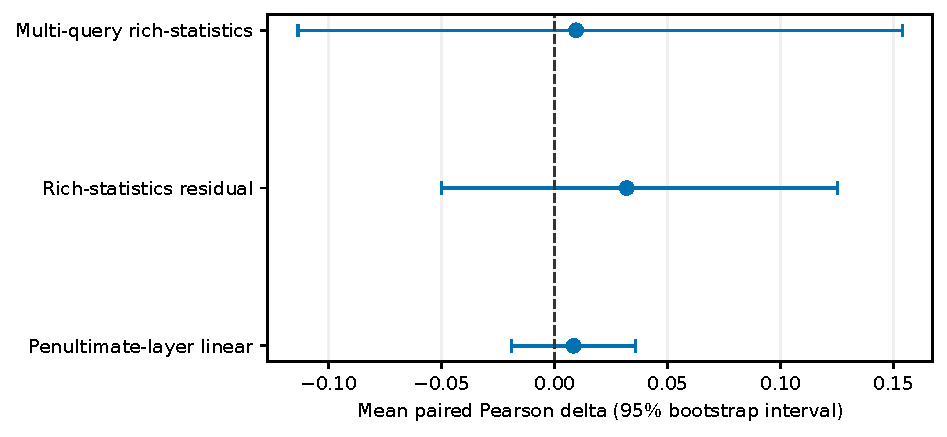
\includegraphics[width=0.82\linewidth]{generated/bootstrap_intervals.pdf}
  \caption{Mean primary Pearson differences and joint 95\% confidence intervals.
  Every interval includes the no-difference line.}
  \label{fig:bootstrap}
\end{figure}

The penultimate-layer and rich-statistics heads improved on every seed. The
multi-query head improved on eight seeds and lost on \MultiQueryLosses{}.
Figure~\ref{fig:seed-deltas} shows these differences. The consistent signs in
the first two comparisons describe training variability on this cohort;
they do not remove uncertainty across participants.

\begin{figure}[tbp]
  \centering
  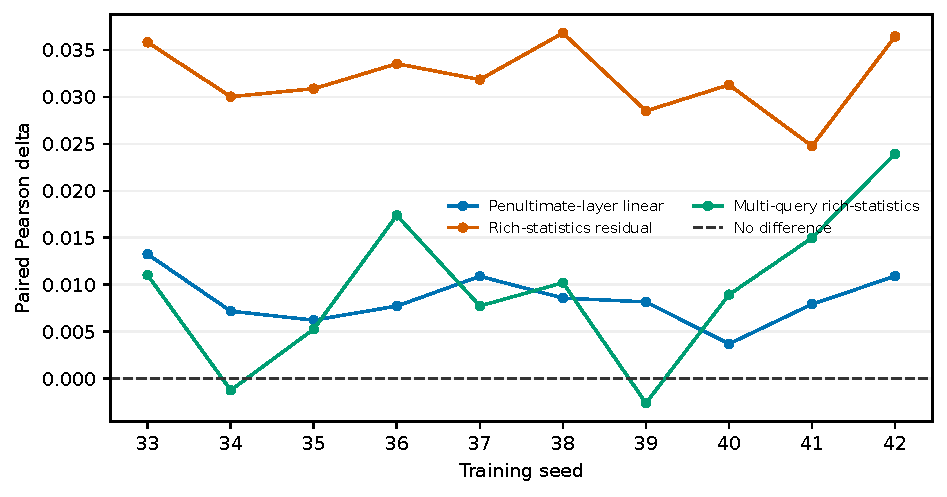
\includegraphics[width=0.86\linewidth]{generated/seed_deltas.pdf}
  \caption{Primary paired Pearson differences by training seed, all evaluated
  on the same 75 participants. Positive values favor the candidate.}
  \label{fig:seed-deltas}
\end{figure}

\subsection{Exploratory training-size analysis}
The 90 runs at 200, 400, and 800 HBN training subjects produced 6,750 predictions
for the same 75 MIPDB participants. Both the rich-statistics and matched MLP
heads had positive mean advantages at every size, with all ten seed differences
positive in each comparison (Figure~\ref{fig:capacity-main}). Their mean
advantages decreased across the tested sizes. The 200-subject intervals were
above zero, while the 800-subject intervals included zero.

Comparing those interval decisions alone does not test whether the effects
changed. Direct 800-minus-200 contrasts were $-0.046$ for the rich head
(95\% CI $[-0.112,0.023]$) and $-0.039$ for the MLP
($[-0.090,0.012]$). Both included zero. One adjacent MLP contrast, 800 minus
400, had an interval below zero ($[-0.061,-0.004]$); its one-sided test of a
positive change gave an adjusted p-value of 1.000. These exploratory results
are reported in full in Appendix~\ref{sec:capacity}; they do not establish a
universal scaling law.

\begin{figure}[tbp]
  \centering
  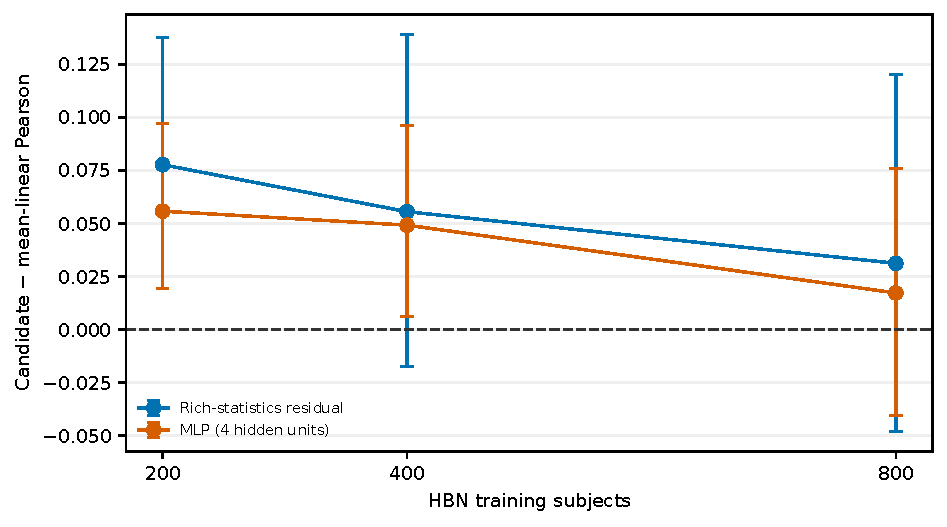
\includegraphics[width=0.86\linewidth]{presentation/capacity_data_regime_delta.pdf}
  \caption{Exploratory training-size analysis. Mean paired Pearson differences
  from the size-matched linear baseline, with joint 95\% intervals.}
  \label{fig:capacity-main}
\end{figure}

\subsection{Exploratory layer-wise analysis}
Four linear probes were evaluated across ten seeds on the same
\LayerwiseSubjectCount{} MIPDB participants. Relative to the final-layer
mean-linear baseline, the mean differences were \LayerwiseMFourDelta{},
\LayerwiseMThreeDelta{}, and \LayerwiseMTwoDelta{} at layers $-4$, $-3$, and
$-2$, respectively. All intervals crossed zero (Table~\ref{tab:layerwise}).
The positive estimates do not establish a stable layer advantage or a primary
superiority claim. Figures~\ref{fig:layerwise-depth} and
\ref{fig:layerwise-seed-deltas} in the appendix show the depth and seed patterns.

\begin{table}[tbp]
  \centering
  \small
  \caption{Exploratory layer-wise differences from the final-layer baseline.
  Intervals resample seeds and participants; Holm-adjusted p-values refer to
  seed sign-flip tests.}
  \label{tab:layerwise}
  \begin{tabular}{lrrrrr}
\toprule
Layer & Mean $\Delta r$ & 95\% interval & Holm $p$ & W/T/L & Worst $\Delta r$ \\
\midrule
Layer -4 & 0.042 & [-0.046, 0.151] & 0.003 & 10/0/0 & 0.031 \\
Layer -3 & 0.030 & [-0.015, 0.084] & 0.003 & 10/0/0 & 0.024 \\
Layer -2 & 0.008 & [-0.019, 0.036] & 0.003 & 10/0/0 & 0.004 \\
\bottomrule
\end{tabular}

\end{table}

\subsection{Secondary transfer to ds006780}
The secondary transfer evaluated \DsRunCount{} selected runs on
\DsSubjectCount{} participants, producing \DsPredictionCount{} predictions.
At 200 HBN training subjects, the rich-statistics head had a mean Pearson
difference of \DsSecondaryDelta{} from the baseline, with 95\% interval
[\DsSecondaryCILow{},\,\DsSecondaryCIHigh{}]. At 800 training subjects, the
difference was \DsPrimaryDelta{} and all \DsPrimaryWins{} seed differences
were positive, but its interval also included zero:
[\DsPrimaryCILow{},\,\DsPrimaryCIHigh{}].

The 800-subject interval width was \DsPrimaryCIWidth{}, exceeding the planned
maximum of \DsPrecisionMaxWidth{}. Thus the precision gate failed. The interval
both leaves the direction of the population advantage uncertain and is wider
than intended; this analysis does not establish stable superiority.
Table~\ref{tab:ds006780-summary} and Figure~\ref{fig:ds006780} report the results.

\begin{table}[tbp]
  \centering
  \small
  \caption{Secondary ds006780 transfer. Pearson and seed SD summarize ten
  training runs. Paired differences and joint intervals compare the rich head
  with the baseline at the same training size.}
  \label{tab:ds006780-summary}
  \begin{tabular}{llrrrr}
\toprule
Training $n$ & Head & Pearson & Seed SD & $\Delta r$ & 95\% interval \\
\midrule
200 & Mean-pooled linear & 0.2650 & 0.0141 & -- & -- \\
200 & Rich-statistics residual & 0.2577 & 0.0168 & -0.0073 & [-0.0861, 0.0721] \\
800 & Mean-pooled linear & 0.3255 & 0.0091 & -- & -- \\
800 & Rich-statistics residual & 0.3543 & 0.0107 & 0.0287 & [-0.0349, 0.0922] \\
\midrule
\multicolumn{6}{l}{Precision gate: failed; observed width 0.1272, threshold 0.0600.} \\
\bottomrule
\end{tabular}

\end{table}

\begin{figure}[tbp]
  \centering
  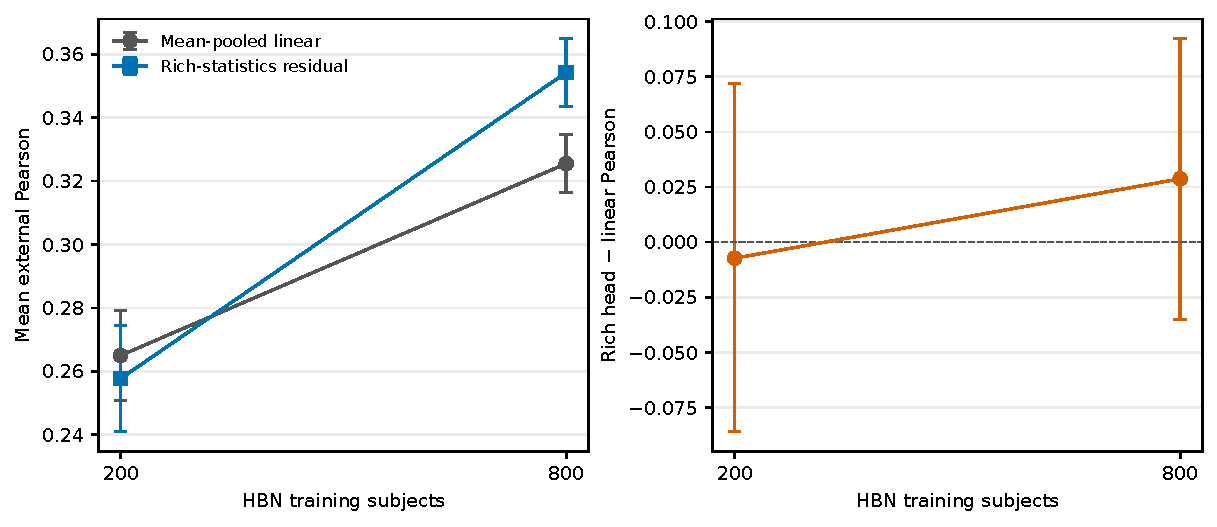
\includegraphics[width=0.95\linewidth]{../results/extensions/ds006780_external_v5/ds006780_external.pdf}
  \caption{Secondary ds006780 results. Left: Pearson correlations with standard
  deviations across seeds. Right: paired differences with intervals that also
  resample participants. Both intervals include zero.}
  \label{fig:ds006780}
\end{figure}


\section{Discussion}

All three primary candidates had higher mean correlations than the baseline,
but every confidence interval included zero. The layer-$-2$ and rich-statistics
heads improved on every seed. Their consistency across training runs did not
resolve uncertainty about the external participants.

The sign-flip tests and bootstrap intervals describe different sources of
variation. The former compare training runs on the fixed MIPDB cohort; the
latter also change which participants enter the evaluation. Small seed-level
p-values can therefore coexist with wide intervals when the estimated
advantage depends on the people being evaluated. Ten seeds provide ten training
runs, not ten independently recruited external cohorts.

\paragraph{The metric changes the preferred head.}
The rich-statistics head had the highest mean Pearson correlation
(\RichResidualPearson{}), whereas the multi-query head had the lowest MAE
(\MultiQueryMAE{} years). Pearson measures association, not agreement in years.
All four heads had negative external $R^2$, and their calibration slopes
exceeded one. Thus a moderate correlation did not imply accurate or
well-calibrated age estimates. These descriptive differences are useful for
understanding the heads, but they were not substituted for the prespecified
endpoint.

\paragraph{More training data did not yield a larger observed advantage.}
In the training-size analysis, the richer heads' mean advantages on MIPDB were
smaller at 800 training subjects than at 200. The endpoint confidence intervals
included zero, so this pattern alone does not establish that the advantage
shrinks with more data. Additional training data may improve the baseline and
candidate together; transfer between cohorts may also limit either predictor.
The experiment does not isolate these explanations. Choosing a new training
size from its MIPDB score would require a fresh external test.

The layer-wise analysis likewise found higher point estimates before the final
layer, but no interval excluded zero. The separate ds006780 transfer produced
a different training-size pattern: the rich head was below the baseline at
200 subjects and above it at 800. At 800, all ten differences were positive,
but the interval again included zero and exceeded the planned width. This
second cohort extends the comparison to another acquisition setting without
establishing a reliable advantage.

\paragraph{Implications.}
A frozen-encoder score describes an encoder used with a particular head,
training set, and metric. Reporting these choices, absolute prediction errors,
and participant-aware intervals makes comparisons easier to interpret. Our
primary, training-size, and layer-wise MIPDB analyses all reuse the same
participants; only the ds006780 extension adds a separate cohort. A larger
external evaluation with a protocol fixed in advance would test whether the
observed gains persist. Evaluating another encoder would address a different
question: how specific these findings are to REVE.

\section{Limitations}

The primary external cohort contains 75 participants. Differences between HBN
and MIPDB in recruitment, age distribution, hardware, and recording procedures
are combined in the observed transfer performance; this design cannot identify
a single source of error. The minimum sample-size threshold did not guarantee
precise estimates. Intervals that include zero leave room for both useful gains
and worse performance, and no equivalence margin was specified.

The main comparison covers one REVE checkpoint, four heads, and ten seeds under
common training settings. Equal budgets do not guarantee that each head was
optimally tuned. The training-size analysis covers three nested subsets, and
the layer-wise analysis covers four depths with separately fitted linear heads.
Both reuse MIPDB after the primary evaluation. These results do not establish a
scaling law or a general ranking of encoders, layers, or heads.

The ds006780 extension uses a separate cohort but was motivated by earlier
results. Its reference was undocumented and its electrode positions were
approximated by a canonical BioSemi montage. The source dataset includes a
sibling group. Family links were not retained in the aggregate evidence, so we
could not establish whether related participants entered the selected sample.
The bootstrap treats participants as independent; any unaccounted family
clustering could make its intervals too narrow. A family-aware sensitivity
analysis would require the original cohort metadata.

The HBN source manifest records age and split membership but not sex or
diagnostic group, limiting the assessment of sampling imbalance. We recovered
the selected ds006780 sample description from public metadata and verified its
participant and age hashes. These checks do not recover the original prediction
vectors or execution caches. Independent recalculation of participant-level
metrics requires those artifacts or a rerun using the original data.

MIPDB participants outside the HBN training-age range were excluded from the
primary analysis. REVE's published pretraining inventory includes HBN releases,
so HBN is not an encoder-unseen evaluation. Although the inventory does not name
MIPDB, we could not independently verify complete absence of pretraining overlap.
We make no encoder-unseen claim for ds006780 either. Finally, predicting
chronological age does not validate a clinical brain-age biomarker.

\section{Conclusion}

Richer heads changed age-prediction performance from frozen REVE features, but
none established a reliable Pearson gain in the primary MIPDB comparison.
Positive differences across training seeds coexisted with confidence intervals
that included zero when participants were also resampled. The highest-correlation
head was not the lowest-error head. Exploratory changes in training size and
layer, and secondary transfer to ds006780, further showed that the comparison
depends on the evaluation setting. These findings support reporting the head,
training data, metric, and uncertainty across participants together. They do
not establish equivalence between the tested heads or rule out gains in other
settings.

\section{Code and Data Availability}

The original research archive is \url{https://github.com/dkozynko/reve-eeg-age-paper}.
It contains the analysis code, executable protocols, validation tests, aggregate
results, and manuscript build instructions. Primary, training-size, layer-wise,
and ds006780 results are stored separately. The reproduction guide explains
which outputs can be rebuilt from these summaries and which require the
original data and execution artifacts.

The primary protocol and selected checkpoints were locked before external
inference, and analysis required a complete prediction inventory. Artifact
hashes allow the retained outputs to be checked against that record; they are
not a public timestamped preregistration. Appendix~\ref{sec:audit} describes
these checks. The repository also retains the HBN source split manifest;
a recovery note documents its identity check and the ds006780 metadata checks.
Raw EEG, participant-level prediction vectors, representation caches, and
checkpoints are not redistributed. Consequently, rebuilding the
published tables and figures is possible from the aggregate bundle, whereas
recomputing the participant-level metrics requires access to the original
artifacts and datasets.

\begingroup
\small
\bibliographystyle{unsrtnat}
\bibliography{references}
\endgroup
\clearpage
\appendix
\section{Protocol and Reproduction Details}
\label{sec:audit}

\subsection{Study record}
Before the primary MIPDB evaluation, a study lock recorded the encoder,
preprocessing, statistical specification, HBN manifests, external cohort,
training environment, and all 40 selected checkpoints. Evaluation recorded its
start before extracting features for primary participants. Existing valid
predictions could not be overwritten, and resumed runs had to use the same
inputs. Analysis required exactly one prediction for each head, seed, and
participant: 3,000 predictions in total.

The compact evidence records the primary analysis hash
\texttt{\SourceAnalysisHash} and prediction-inventory hash
\texttt{\PredictionInventoryHash}. These identify the retained result and its
source inventory. They do not replace access to the inventory or provide an
independent public timestamp for the protocol.

The source analyses, figures, and tables are linked by file manifests. Numeric
commands in the manuscript are generated from aggregate results. The editorial
presentation assets use the same retained values with shorter labels; their
manifest records their source files separately. Rebuilding those assets does
not rerun participant-level inference.

\subsection{Interpretation of the decision rule}
The five primary conditions serve different purposes. The minimum cohort size
sets a floor on the evaluation sample. Holm correction addresses the three
seed-level tests, while the bootstrap lower bound requires a positive estimate
when seeds and participants are resampled. The win count and worst-seed floor
limit dependence on favorable training runs. No candidate passed the bootstrap
condition. The multi-query head lost on two seeds, but still met the eight-win
and worst-seed thresholds. Passing those thresholds did not compensate for an
interval containing zero.

\subsection{Earlier and later analyses}
Previously inspected HBN R5 screens motivated candidate families but are
retrospective evidence. NeuralBench-compatible end-to-end runs update the
encoder and provide implementation context, not frozen-probe scores. Neither
is part of the primary MIPDB effect estimate.

The training-size and layer-wise follow-ups reuse the MIPDB cohort after its
first evaluation. Their separate protocol records preserve what was run but
cannot make those participants an untouched holdout again. The ds006780
transfer adds a separate cohort and uses the configuration recorded in
\texttt{configs/research/ds006780\_external\_transfer.json}. Its configuration
hash matches the v5 aggregate execution record, including dataset version
1.0.0 and the pinned source revision. It remains secondary because the
comparison was motivated by earlier findings.

\subsection{Additional primary and layer-wise figures}
Figure~\ref{fig:calibration} summarizes calibration. Figures~\ref{fig:layerwise-depth}
and \ref{fig:layerwise-seed-deltas} show the exploratory depth comparison.

\begin{figure}[!htbp]
  \centering
  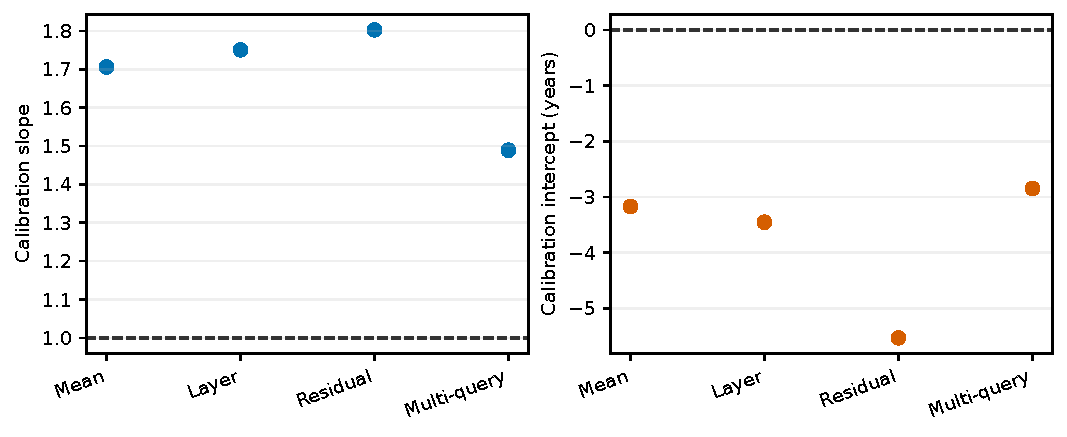
\includegraphics[width=0.80\linewidth]{generated/calibration_summary.pdf}
  \caption{Mean MIPDB calibration slopes and intercepts across seeds. Dashed
  lines mark one and zero, respectively. Calibration regresses observed age on
  predicted age; no external recalibration was applied.}
  \label{fig:calibration}
\end{figure}

\begin{figure}[!htbp]
  \centering
  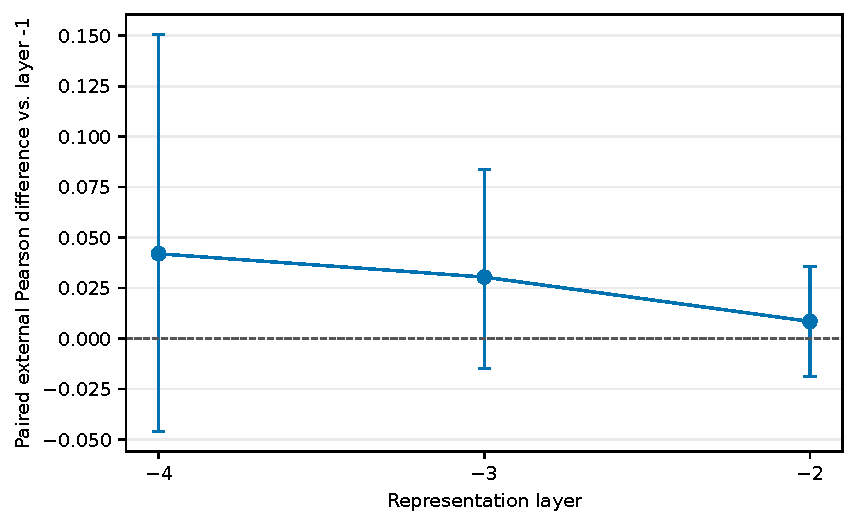
\includegraphics[width=0.80\linewidth]{../results/extensions/layerwise_probe_20260910/assets/layerwise_depth.pdf}
  \caption{Exploratory layer-wise differences from the final layer, with joint
  seed-and-participant intervals. All intervals include zero.}
  \label{fig:layerwise-depth}
\end{figure}

\begin{figure}[!htbp]
  \centering
  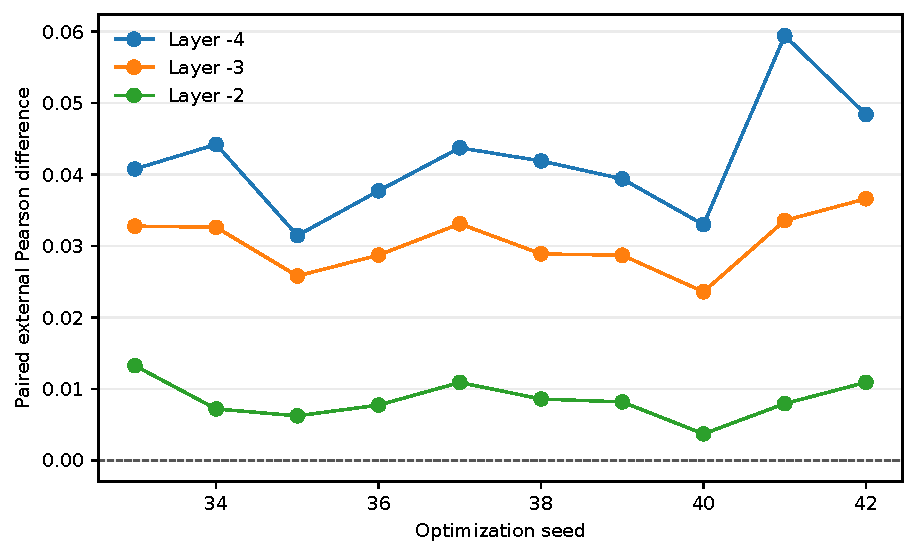
\includegraphics[width=0.80\linewidth]{../results/extensions/layerwise_probe_20260910/assets/layerwise_seed_deltas.pdf}
  \caption{Paired layer-wise Pearson differences across seeds on the same
  MIPDB participants.}
  \label{fig:layerwise-seed-deltas}
\end{figure}

\clearpage
\section{Training-Size Analysis}
\label{sec:capacity}

This exploratory analysis used three heads, three nested HBN training subsets,
and ten seeds, for 90 runs. Each selected checkpoint was evaluated on the same
75 MIPDB participants. The resulting 6,750 predictions are repeated evaluations
of those participants, not independent observations.

\subsection{Absolute performance and paired differences}
Table~\ref{tab:capacity-absolute} reports absolute correlations and parameter
counts. Table~\ref{tab:capacity-cells} gives candidate differences from the
size-matched baseline. The richer heads improved on all ten seeds in each cell.
Both 200-subject intervals and the MLP's 400-subject interval excluded zero;
the other intervals included zero.

\begin{table}[!htbp]
  \centering
  \small
  \caption{MIPDB correlations by HBN training size. SD is computed across ten
  seeds. The MLP has four hidden units.}
  \label{tab:capacity-absolute}
  \begin{tabular}{llrrr}
\toprule
Train $n$ & Head & Params & Mean Pearson & Seed SD \\
\midrule
200 & Mean-linear baseline & 513 & 0.527 & 0.011 \\
200 & Rich statistics & 2561 & 0.604 & 0.009 \\
200 & MLP (4 units) & 2569 & 0.582 & 0.025 \\
400 & Mean-linear baseline & 513 & 0.655 & 0.008 \\
400 & Rich statistics & 2561 & 0.711 & 0.008 \\
400 & MLP (4 units) & 2569 & 0.704 & 0.014 \\
800 & Mean-linear baseline & 513 & 0.645 & 0.008 \\
800 & Rich statistics & 2561 & 0.676 & 0.007 \\
800 & MLP (4 units) & 2569 & 0.662 & 0.012 \\
\bottomrule
\end{tabular}

\end{table}

\begin{table}[!htbp]
  \centering
  \small
  \caption{Paired candidate differences at each training size. W/T/L counts
  positive, zero, and negative seed differences. Intervals resample seeds and
  participants; p-values are exploratory.}
  \label{tab:capacity-cells}
  \begin{tabular}{rlrrrrr}
\toprule
Train $n$ & Head & Params & Mean $\Delta$ & 95\% CI & Holm $p$ & W/T/L \\
\midrule
200 & Rich statistics & 2561 & 0.078 & [0.019, 0.138] & 0.006 & 10/0/0 \\
400 & Rich statistics & 2561 & 0.056 & [-0.017, 0.139] & 0.006 & 10/0/0 \\
800 & Rich statistics & 2561 & 0.031 & [-0.048, 0.120] & 0.006 & 10/0/0 \\
200 & MLP (4 units) & 2569 & 0.056 & [0.019, 0.097] & 0.006 & 10/0/0 \\
400 & MLP (4 units) & 2569 & 0.049 & [0.006, 0.096] & 0.006 & 10/0/0 \\
800 & MLP (4 units) & 2569 & 0.017 & [-0.040, 0.076] & 0.006 & 10/0/0 \\
\bottomrule
\end{tabular}

\end{table}

\subsection{Changes in the candidate advantage}
Table~\ref{tab:capacity-contrasts} compares paired advantages between training
sizes. For example, 800 minus 200 subtracts the candidate's advantage at 200
subjects from its advantage at 800. All observed changes were negative. The
one-sided sign-flip tests retained the prespecified positive-change alternative,
which explains their large p-values; they are not tests for any change in
either direction. Only the MLP's 800-minus-400 bootstrap interval excluded zero.
The endpoint intervals included zero for both heads.

\begin{table}[!htbp]
  \centering
  \small
  \caption{Exploratory changes in the paired Pearson advantage. A negative
  value means a smaller candidate advantage at the larger training size.
  Holm p-values test the positive direction; SD describes seed differences.}
  \label{tab:capacity-contrasts}
  \begin{tabular}{llrrrr}
\toprule
Head & Contrast & Change in $\Delta$ & 95\% CI & Holm $p$ & SD \\
\midrule
Rich statistics & 800 minus 200 & -0.046 & [-0.112, 0.023] & 1.000 & 0.010 \\
Rich statistics & 400 minus 200 & -0.022 & [-0.069, 0.031] & 1.000 & 0.008 \\
Rich statistics & 800 minus 400 & -0.024 & [-0.065, 0.016] & 1.000 & 0.005 \\
MLP (4 units) & 800 minus 200 & -0.039 & [-0.090, 0.012] & 1.000 & 0.018 \\
MLP (4 units) & 400 minus 200 & -0.007 & [-0.044, 0.029] & 1.000 & 0.014 \\
MLP (4 units) & 800 minus 400 & -0.032 & [-0.061, -0.004] & 1.000 & 0.008 \\
\bottomrule
\end{tabular}

\end{table}

Table~\ref{tab:capacity-transfer} shows HBN validation and MIPDB correlations for
the selected candidate checkpoints. External scores did not select checkpoints.
Figure~\ref{fig:capacity-absolute} shows absolute performance, and
Figure~\ref{fig:capacity-seed-deltas} shows individual seed differences.
The joint intervals are shown once in Figure~\ref{fig:capacity-main}.

\begin{table}[!htbp]
  \centering
  \small
  \caption{HBN validation and MIPDB correlations for selected candidate heads,
  averaged over seeds.}
  \label{tab:capacity-transfer}
  \begin{tabular}{llrr}
\toprule
Train $n$ & Head & HBN validation $r$ & MIPDB $r$ \\
\midrule
200 & Rich statistics & 0.645 & 0.604 \\
400 & Rich statistics & 0.711 & 0.711 \\
800 & Rich statistics & 0.736 & 0.676 \\
200 & MLP (4 units) & 0.648 & 0.582 \\
400 & MLP (4 units) & 0.741 & 0.704 \\
800 & MLP (4 units) & 0.742 & 0.662 \\
\bottomrule
\end{tabular}

\end{table}

\begin{figure}[!htbp]
  \centering
  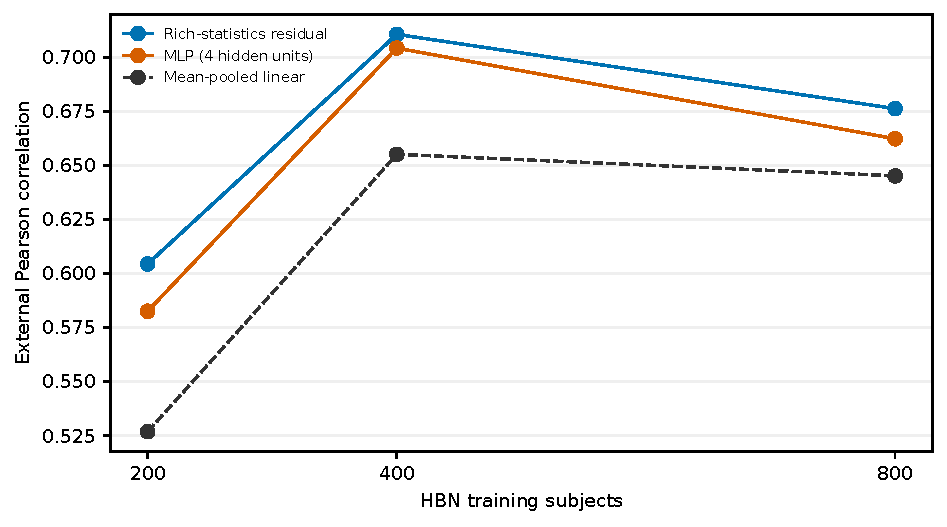
\includegraphics[width=0.80\linewidth]{presentation/capacity_data_regime_absolute.pdf}
  \caption{Absolute MIPDB correlations for each training size and head.}
  \label{fig:capacity-absolute}
\end{figure}

\begin{figure}[!htbp]
  \centering
  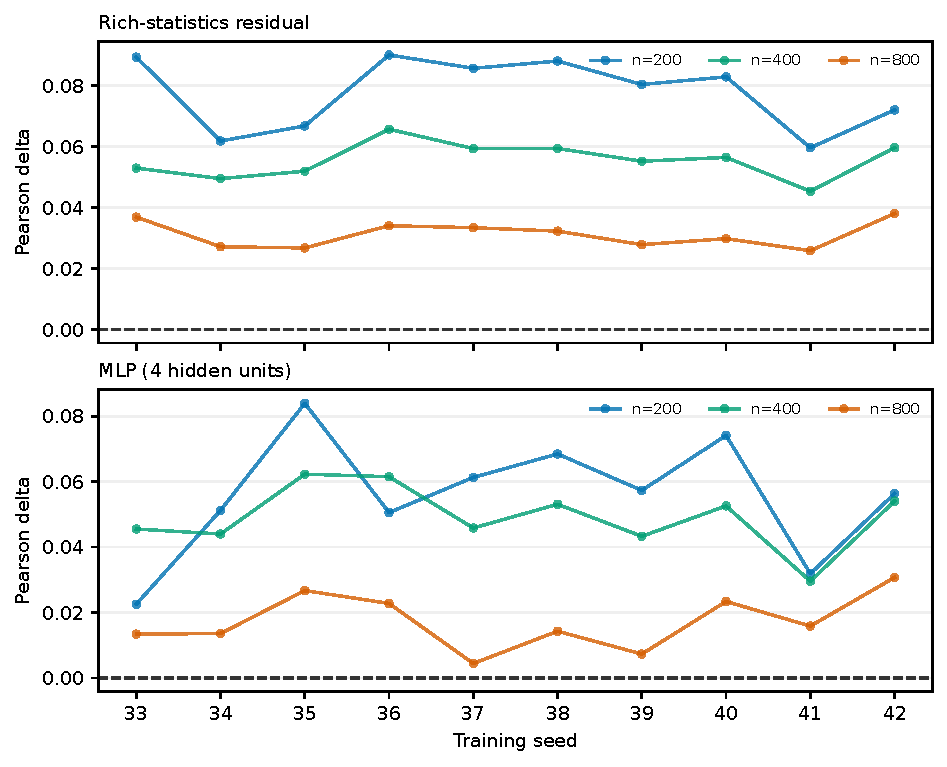
\includegraphics[width=0.80\linewidth]{presentation/capacity_data_regime_seed_deltas.pdf}
  \caption{Paired Pearson differences for the rich-statistics and four-unit
  MLP heads across seeds and HBN training sizes.}
  \label{fig:capacity-seed-deltas}
\end{figure}


\end{document}
